\section*{Variational Autoencoders}

The history of Variational Autoencoders could be summarised by sequentially looking into the following papers:

\begin{itemize}
    \item An and Cho, 2015. Variational autoencoder based anomaly detection using reconstruction probability.
    \item Xu et al., 2018. Unsupervised anomaly detection via variational autoencoder for seasonal KPIs in web applications
    \item Zimmerer et al., 2019. Unsupervised anomaly localization using variational auto-encoders.
\end{itemize}

The first paper must be used to understand the differences between Autoencoders and Variational Autoencoders. This is important since VAE can be interpreted as a new technique with origin on Autoencoders, thus, sharing fundamentals and architectures.

An and Cho, described a VAE as "a probabilistic graphical model that combines variational inference with deep learning”. Because VAE reduces dimensions in a probabilistically sound way, theoretical foundations are firm. The advantage of a VAE over an autoencoder and a PCA is that it provides a probability measure rather than a reconstruction error as an anomaly score, which we will call the reconstruction probability. Probabilities are more principled and objective than reconstruction errors and does not require model specific thresholds for judging anomalies."

In other words, Jeremy Jordan describes the same in simpler words "A variational autoencoder provides a probabilistic manner for describing an observation in latent space. Thus, rather than building an encoder which outputs a single value to describe each latent state attribute, we'll formulate our encoder to describe a probability distribution for each latent attribute.".

\begin{figure}[ht]
    \hspace*{-1in}
    \centering
    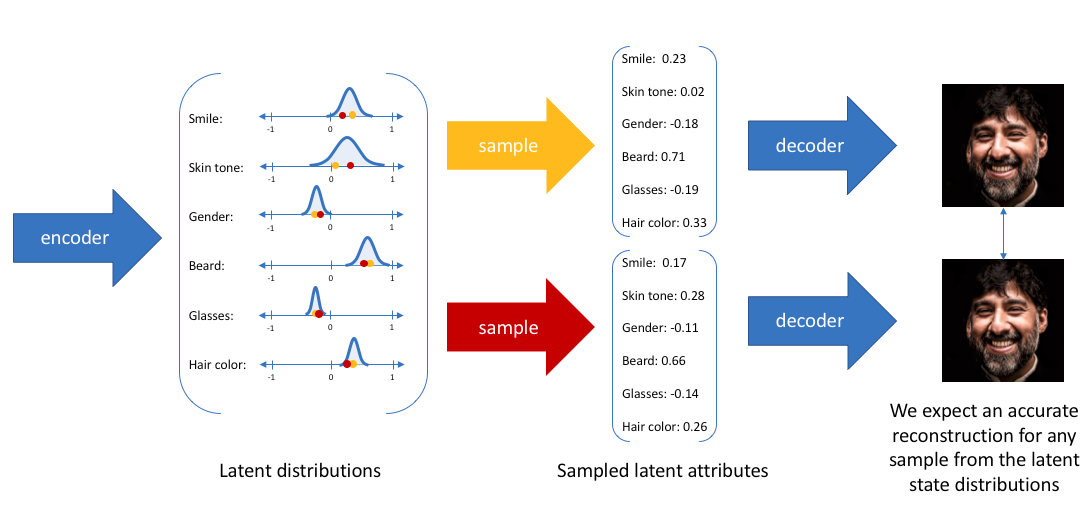
\includegraphics[width = 17cm, height = 8cm]{images/vaes.png}
    \caption[]{Variational Autoencoders by Jerermy Jordan}
    \label{fig:vaes}
\end{figure}

An and Cho conclude "To summarize, it is the distribution parameters that are being modeled in the VAE, not the value itself."

To understand the differences between Autoencoders and VAEs, An and Cho listed 3 differences:

\begin{enumerate}
    \item VAE latent space are stochastic variables, not deterministic ones
    \item Reconstruction in VAE adds the variability of the reconstruction by considering the variance parameter of the distribution function.
    \item Autoencoders use reconstruction errors as anomaly score, while VAE reconstructions are probability measures which work best for heterogeneous data and deciding the reconstruction probability threshold is easier and more objective than deciding for reconstruction error.
\end{enumerate}

Finally, An and Cho proved that VAE outperformed autoencoders and PCA based methods on 2 different popular datasets, MNIST and KDD.

Xu et al. later proved the same on a large internet company dataset that shows a combination of seasonal patterns with local variations and the statistics of the Gaussian noises.

The project consisted of detecting anomalies on Key Performance Indicators on a website; KPIs are time series data measuring metrics such as number of connected users, transactions or orders. Websites for retail industry follow a seasonal distribution and a local variation that explains the increasing trend over days.

Finally, Zimmerer et al., 2018 proved that VAEs could keep the assumption-free principle by improving the used network architecture with a combination of the reconstruction term with the density-based anomaly scoring. Before, the VAEs had shown great potential on unsupervised learning of data distributions but required modifications on the model architecture to perform well for the problem seen during the evaluation, which breaks the assumption-free principle. 

In detail, VAE can approximate data distributions by optimizing a lower bound, often termed evidence lower bound (ELBO) which is usually employed as a proxy to compare the likelihood. ELBO is a combination of the reconstruction error and the Kullback-Leibler (KL)-divergence, a backpropagation mechanism. This combination is called a context-encoder VAE or ceVAE.
